\documentclass[twoside]{book}

% Packages required by doxygen
\usepackage{fixltx2e}
\usepackage{calc}
\usepackage{doxygen}
\usepackage[export]{adjustbox} % also loads graphicx
\usepackage{graphicx}
\usepackage[utf8]{inputenc}
\usepackage{makeidx}
\usepackage{multicol}
\usepackage{multirow}
\PassOptionsToPackage{warn}{textcomp}
\usepackage{textcomp}
\usepackage[nointegrals]{wasysym}
\usepackage[table]{xcolor}

% Font selection
\usepackage[T1]{fontenc}
\usepackage[scaled=.90]{helvet}
\usepackage{courier}
\usepackage{amssymb}
\usepackage{sectsty}
\renewcommand{\familydefault}{\sfdefault}
\allsectionsfont{%
  \fontseries{bc}\selectfont%
  \color{darkgray}%
}
\renewcommand{\DoxyLabelFont}{%
  \fontseries{bc}\selectfont%
  \color{darkgray}%
}
\newcommand{\+}{\discretionary{\mbox{\scriptsize$\hookleftarrow$}}{}{}}

% Page & text layout
\usepackage{geometry}
\geometry{%
  a4paper,%
  top=2.5cm,%
  bottom=2.5cm,%
  left=2.5cm,%
  right=2.5cm%
}
\tolerance=750
\hfuzz=15pt
\hbadness=750
\setlength{\emergencystretch}{15pt}
\setlength{\parindent}{0cm}
\setlength{\parskip}{3ex plus 2ex minus 2ex}
\makeatletter
\renewcommand{\paragraph}{%
  \@startsection{paragraph}{4}{0ex}{-1.0ex}{1.0ex}{%
    \normalfont\normalsize\bfseries\SS@parafont%
  }%
}
\renewcommand{\subparagraph}{%
  \@startsection{subparagraph}{5}{0ex}{-1.0ex}{1.0ex}{%
    \normalfont\normalsize\bfseries\SS@subparafont%
  }%
}
\makeatother

% Headers & footers
\usepackage{fancyhdr}
\pagestyle{fancyplain}
\fancyhead[LE]{\fancyplain{}{\bfseries\thepage}}
\fancyhead[CE]{\fancyplain{}{}}
\fancyhead[RE]{\fancyplain{}{\bfseries\leftmark}}
\fancyhead[LO]{\fancyplain{}{\bfseries\rightmark}}
\fancyhead[CO]{\fancyplain{}{}}
\fancyhead[RO]{\fancyplain{}{\bfseries\thepage}}
\fancyfoot[LE]{\fancyplain{}{}}
\fancyfoot[CE]{\fancyplain{}{}}
\fancyfoot[RE]{\fancyplain{}{\bfseries\scriptsize Generated by Doxygen }}
\fancyfoot[LO]{\fancyplain{}{\bfseries\scriptsize Generated by Doxygen }}
\fancyfoot[CO]{\fancyplain{}{}}
\fancyfoot[RO]{\fancyplain{}{}}
\renewcommand{\footrulewidth}{0.4pt}
\renewcommand{\chaptermark}[1]{%
  \markboth{#1}{}%
}
\renewcommand{\sectionmark}[1]{%
  \markright{\thesection\ #1}%
}

% Indices & bibliography
\usepackage{natbib}
\usepackage[titles]{tocloft}
\setcounter{tocdepth}{3}
\setcounter{secnumdepth}{5}
\makeindex

% Hyperlinks (required, but should be loaded last)
\usepackage{ifpdf}
\ifpdf
  \usepackage[pdftex,pagebackref=true]{hyperref}
\else
  \usepackage[ps2pdf,pagebackref=true]{hyperref}
\fi
\hypersetup{%
  colorlinks=true,%
  linkcolor=blue,%
  citecolor=blue,%
  unicode%
}

% Custom commands
\newcommand{\clearemptydoublepage}{%
  \newpage{\pagestyle{empty}\cleardoublepage}%
}

\usepackage{caption}
\captionsetup{labelsep=space,justification=centering,font={bf},singlelinecheck=off,skip=4pt,position=top}

%===== C O N T E N T S =====

\begin{document}

% Titlepage & ToC
\hypersetup{pageanchor=false,
             bookmarksnumbered=true,
             pdfencoding=unicode
            }
\pagenumbering{alph}
\begin{titlepage}
\vspace*{7cm}
\begin{center}%
{\Large I\+V\+S-\/\+Projekt 2 }\\
\vspace*{1cm}
{\large Generated by Doxygen 1.8.14}\\
\end{center}
\end{titlepage}
\clearemptydoublepage
\pagenumbering{roman}
\tableofcontents
\clearemptydoublepage
\pagenumbering{arabic}
\hypersetup{pageanchor=true}

%--- Begin generated contents ---
\chapter{Namespace Index}
\section{Packages}
Here are the packages with brief descriptions (if available)\+:\begin{DoxyCompactList}
\item\contentsline{section}{\mbox{\hyperlink{namespace_i_v_s}{I\+VS}} }{\pageref{namespace_i_v_s}}{}
\item\contentsline{section}{\mbox{\hyperlink{namespace_i_v_s_1_1_properties}{I\+V\+S.\+Properties}} }{\pageref{namespace_i_v_s_1_1_properties}}{}
\item\contentsline{section}{\mbox{\hyperlink{namespace_math_library}{Math\+Library}} }{\pageref{namespace_math_library}}{}
\item\contentsline{section}{\mbox{\hyperlink{namespace_smerodatna__odhylka}{Smerodatna\+\_\+odhylka}} }{\pageref{namespace_smerodatna__odhylka}}{}
\end{DoxyCompactList}

\chapter{Hierarchical Index}
\section{Class Hierarchy}
This inheritance list is sorted roughly, but not completely, alphabetically\+:\begin{DoxyCompactList}
\item Form\begin{DoxyCompactList}
\item \contentsline{section}{I\+V\+S.\+Calculator}{\pageref{class_i_v_s_1_1_calculator}}{}
\item \contentsline{section}{I\+V\+S.\+napoveda}{\pageref{class_i_v_s_1_1napoveda}}{}
\item \contentsline{section}{I\+V\+S.\+Testy}{\pageref{class_i_v_s_1_1_testy}}{}
\end{DoxyCompactList}
\item \contentsline{section}{Math\+Library.\+math}{\pageref{class_math_library_1_1math}}{}
\item \contentsline{section}{Smerodatna\+\_\+odhylka.\+Program}{\pageref{class_smerodatna__odhylka_1_1_program}}{}
\end{DoxyCompactList}

\chapter{Class Index}
\section{Class List}
Here are the classes, structs, unions and interfaces with brief descriptions\+:\begin{DoxyCompactList}
\item\contentsline{section}{\mbox{\hyperlink{class_i_v_s_1_1_calculator}{I\+V\+S.\+Calculator}} \\*G\+UI Kalkulacky }{\pageref{class_i_v_s_1_1_calculator}}{}
\item\contentsline{section}{\mbox{\hyperlink{class_math_library_1_1math}{Math\+Library.\+math}} \\*Trida math provadejici zakladni a porkocile mat operace. Umi i zpracovat vyraz bez zavorek. }{\pageref{class_math_library_1_1math}}{}
\item\contentsline{section}{\mbox{\hyperlink{class_i_v_s_1_1napoveda}{I\+V\+S.\+napoveda}} \\*Trida formulare napovedy }{\pageref{class_i_v_s_1_1napoveda}}{}
\item\contentsline{section}{\mbox{\hyperlink{class_smerodatna__odhylka_1_1_program}{Smerodatna\+\_\+odhylka.\+Program}} \\*\mbox{\hyperlink{class_smerodatna__odhylka_1_1_program}{Program}} pro vypocet smerodatne odchylky z cisel nactenych na stdin }{\pageref{class_smerodatna__odhylka_1_1_program}}{}
\item\contentsline{section}{\mbox{\hyperlink{class_i_v_s_1_1_testy}{I\+V\+S.\+Testy}} \\*Trida testu }{\pageref{class_i_v_s_1_1_testy}}{}
\end{DoxyCompactList}

\chapter{Namespace Documentation}
\hypertarget{namespace_i_v_s}{}\section{I\+VS Namespace Reference}
\label{namespace_i_v_s}\index{I\+VS@{I\+VS}}
\subsection*{Namespaces}
\begin{DoxyCompactItemize}
\end{DoxyCompactItemize}
\subsection*{Classes}
\begin{DoxyCompactItemize}
\item 
class \mbox{\hyperlink{class_i_v_s_1_1_calculator}{Calculator}}
\begin{DoxyCompactList}\small\item\em Hlavni form aplikace \end{DoxyCompactList}\item 
class \mbox{\hyperlink{class_i_v_s_1_1napoveda}{napoveda}}
\begin{DoxyCompactList}\small\item\em Trida formulare napovedy \end{DoxyCompactList}\item 
class {\bfseries Program}
\begin{DoxyCompactList}\small\item\em Hlavni vstupni bod aplikace \end{DoxyCompactList}\item 
class \mbox{\hyperlink{class_i_v_s_1_1_testy}{Testy}}
\begin{DoxyCompactList}\small\item\em Trida testu \end{DoxyCompactList}\end{DoxyCompactItemize}

\hypertarget{namespace_i_v_s_1_1_properties}{}\section{I\+V\+S.\+Properties Namespace Reference}
\label{namespace_i_v_s_1_1_properties}\index{I\+V\+S.\+Properties@{I\+V\+S.\+Properties}}
\subsection*{Classes}
\begin{DoxyCompactItemize}
\item 
class {\bfseries Resources}
\begin{DoxyCompactList}\small\item\em Třída prostředků se silnými typy pro vyhledávání lokalizovaných řetězců atp. \end{DoxyCompactList}\item 
class {\bfseries Settings}
\end{DoxyCompactItemize}

\hypertarget{namespace_math_library}{}\section{Math\+Library Namespace Reference}
\label{namespace_math_library}\index{Math\+Library@{Math\+Library}}
\subsection*{Classes}
\begin{DoxyCompactItemize}
\item 
class \mbox{\hyperlink{class_math_library_1_1math}{math}}
\end{DoxyCompactItemize}

\hypertarget{namespace_smerodatna__odhylka}{}\section{Smerodatna\+\_\+odhylka Namespace Reference}
\label{namespace_smerodatna__odhylka}\index{Smerodatna\+\_\+odhylka@{Smerodatna\+\_\+odhylka}}
\subsection*{Classes}
\begin{DoxyCompactItemize}
\item 
class \mbox{\hyperlink{class_smerodatna__odhylka_1_1_program}{Program}}
\begin{DoxyCompactList}\small\item\em \mbox{\hyperlink{class_smerodatna__odhylka_1_1_program}{Program}} pro vypocet smerodatne odchylky z cisel nactenych na stdin \end{DoxyCompactList}\end{DoxyCompactItemize}

\chapter{Class Documentation}
\hypertarget{class_i_v_s_1_1_calculator}{}\section{I\+V\+S.\+Calculator Class Reference}
\label{class_i_v_s_1_1_calculator}\index{I\+V\+S.\+Calculator@{I\+V\+S.\+Calculator}}


Hlavni form aplikace  


Inheritance diagram for I\+V\+S.\+Calculator\+:\begin{figure}[H]
\begin{center}
\leavevmode
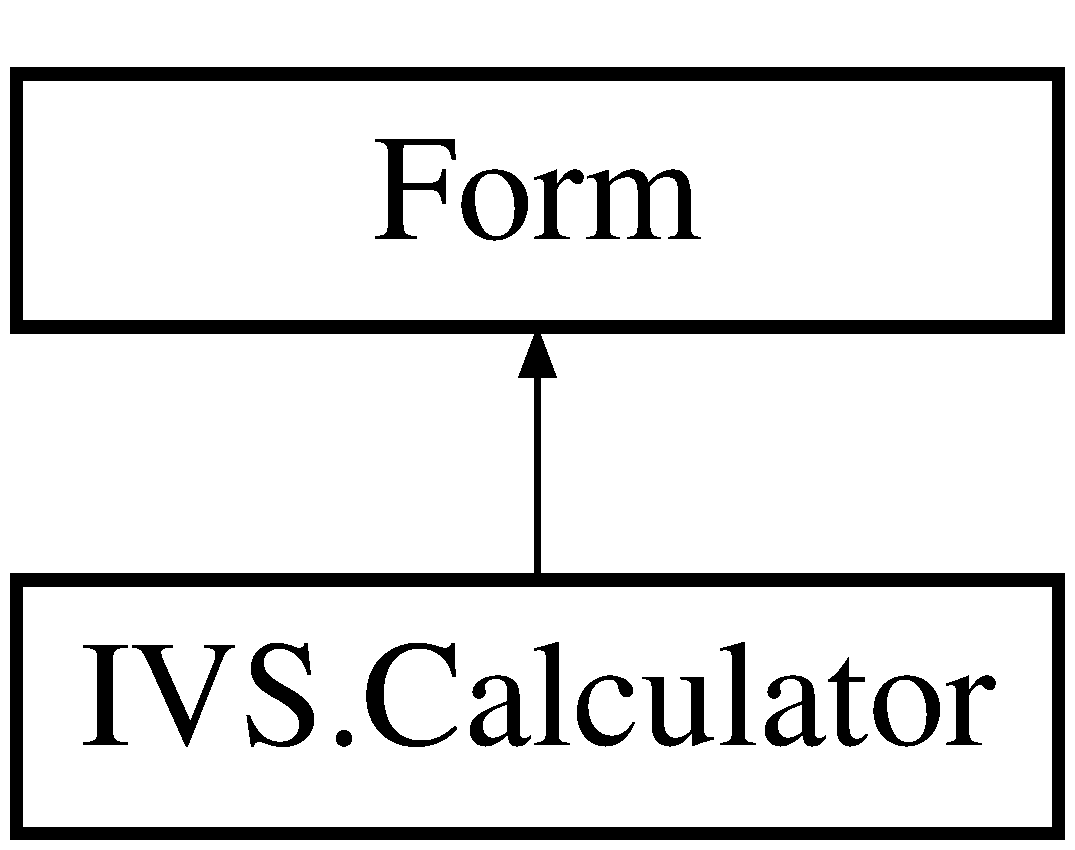
\includegraphics[height=2.000000cm]{class_i_v_s_1_1_calculator}
\end{center}
\end{figure}
\subsection*{Public Member Functions}
\begin{DoxyCompactItemize}
\item 
\mbox{\hyperlink{class_i_v_s_1_1_calculator_a3d3f790c8ecb804fe212427b914dd82f}{Calculator}} ()
\begin{DoxyCompactList}\small\item\em Init komponent \end{DoxyCompactList}\end{DoxyCompactItemize}
\subsection*{Protected Member Functions}
\begin{DoxyCompactItemize}
\item 
void \mbox{\hyperlink{class_i_v_s_1_1_calculator_a3c3a8cab086cf9f773e7b4dbddcbad58}{Calculator\+\_\+\+Load}} (object sender, Event\+Args e)
\begin{DoxyCompactList}\small\item\em Pri nacteni formulare prepne focus na textbox \end{DoxyCompactList}\item 
void \mbox{\hyperlink{class_i_v_s_1_1_calculator_a5b2424094c9a7228f4b71fd9e27a79ca}{text\+Box1\+\_\+\+Text\+Changed}} (object sender, Event\+Args e)
\begin{DoxyCompactList}\small\item\em textbox na zadávanie vstupov \end{DoxyCompactList}\item 
void \mbox{\hyperlink{class_i_v_s_1_1_calculator_ac1763f222a684150c84c3fe98c0820e1}{button4\+\_\+\+Click}} (object sender, Event\+Args e)
\begin{DoxyCompactList}\small\item\em Vloženie \textquotesingle{}0\textquotesingle{} do textového pola \end{DoxyCompactList}\item 
void \mbox{\hyperlink{class_i_v_s_1_1_calculator_a4aab8fcd134875c22735f5c69709f3a9}{button15\+\_\+\+Click}} (object sender, Event\+Args e)
\begin{DoxyCompactList}\small\item\em Vloženie \textquotesingle{}+\textquotesingle{} do textového pola \end{DoxyCompactList}\item 
void \mbox{\hyperlink{class_i_v_s_1_1_calculator_abb0b26c38b19fed222be5905a63db4fa}{button20\+\_\+\+Click}} (object sender, Event\+Args e)
\begin{DoxyCompactList}\small\item\em vloženie \textquotesingle{}(\textquotesingle{} do textového pola \end{DoxyCompactList}\item 
void \mbox{\hyperlink{class_i_v_s_1_1_calculator_acb35f01364be2f89cd6615bfe6b90725}{button1\+\_\+\+Click}} (object sender, Event\+Args e)
\begin{DoxyCompactList}\small\item\em Vloženie \textquotesingle{}1\textquotesingle{} do textového pola \end{DoxyCompactList}\item 
void \mbox{\hyperlink{class_i_v_s_1_1_calculator_aa6a17fb7e856187dfd9b8964e67e2f57}{button2\+\_\+\+Click}} (object sender, Event\+Args e)
\begin{DoxyCompactList}\small\item\em Vloženie \textquotesingle{}2\textquotesingle{} do textového pola \end{DoxyCompactList}\item 
void \mbox{\hyperlink{class_i_v_s_1_1_calculator_a4478858fe2f745473de5b68a7a57b2f3}{button3\+\_\+\+Click}} (object sender, Event\+Args e)
\begin{DoxyCompactList}\small\item\em Vloženie \textquotesingle{}3\textquotesingle{} do textového pola \end{DoxyCompactList}\item 
void \mbox{\hyperlink{class_i_v_s_1_1_calculator_a7ea090e719a196447aadfd4a065a42f0}{button5\+\_\+\+Click}} (object sender, Event\+Args e)
\begin{DoxyCompactList}\small\item\em Vloženie \textquotesingle{}4\textquotesingle{} do textového pola \end{DoxyCompactList}\item 
void \mbox{\hyperlink{class_i_v_s_1_1_calculator_a061c919ebdc08c877ae00f4ce1697739}{button6\+\_\+\+Click}} (object sender, Event\+Args e)
\begin{DoxyCompactList}\small\item\em Vloženie \textquotesingle{}5\textquotesingle{} do textového pola \end{DoxyCompactList}\item 
void \mbox{\hyperlink{class_i_v_s_1_1_calculator_ab96b96bb1f464fa88084118d38bc9d9e}{button7\+\_\+\+Click}} (object sender, Event\+Args e)
\begin{DoxyCompactList}\small\item\em Vloženie \textquotesingle{}6\textquotesingle{} do textového pola \end{DoxyCompactList}\item 
void \mbox{\hyperlink{class_i_v_s_1_1_calculator_a7de16fbeb3e7bea132d8540dde1cd110}{button8\+\_\+\+Click}} (object sender, Event\+Args e)
\begin{DoxyCompactList}\small\item\em Vloženie \textquotesingle{}7\textquotesingle{} do textového pola \end{DoxyCompactList}\item 
void \mbox{\hyperlink{class_i_v_s_1_1_calculator_ad6751dcda5da874d2c4c933020f5bc70}{button9\+\_\+\+Click}} (object sender, Event\+Args e)
\begin{DoxyCompactList}\small\item\em Vloženie \textquotesingle{}8\textquotesingle{} do textového pola \end{DoxyCompactList}\item 
void \mbox{\hyperlink{class_i_v_s_1_1_calculator_aa06324ed88e9004bf9cd91dd9195e146}{button10\+\_\+\+Click}} (object sender, Event\+Args e)
\begin{DoxyCompactList}\small\item\em Vloženie \textquotesingle{}9\textquotesingle{} do textového pola \end{DoxyCompactList}\item 
void \mbox{\hyperlink{class_i_v_s_1_1_calculator_a33dc653a738421ce3fe770c4c470a224}{button21\+\_\+\+Click}} (object sender, Event\+Args e)
\begin{DoxyCompactList}\small\item\em Vloženie \textquotesingle{})\textquotesingle{} do textového pola \end{DoxyCompactList}\item 
void \mbox{\hyperlink{class_i_v_s_1_1_calculator_aabdaceb3733e6b9873224d39ba10aec0}{button22\+\_\+\+Click}} (object sender, Event\+Args e)
\begin{DoxyCompactList}\small\item\em Vyčistenie textového pola \end{DoxyCompactList}\item 
void \mbox{\hyperlink{class_i_v_s_1_1_calculator_a2ec5538328f39267ddd848fbc9200de7}{button19\+\_\+\+Click}} (object sender, Event\+Args e)
\begin{DoxyCompactList}\small\item\em Vloženie \textquotesingle{},\textquotesingle{} do textového pola \end{DoxyCompactList}\item 
void \mbox{\hyperlink{class_i_v_s_1_1_calculator_a8e6a0c70145a0d3bfe53de19b9e980ea}{button16\+\_\+\+Click}} (object sender, Event\+Args e)
\begin{DoxyCompactList}\small\item\em Vloženie \textquotesingle{}-\/\textquotesingle{} do textového pola \end{DoxyCompactList}\item 
void \mbox{\hyperlink{class_i_v_s_1_1_calculator_a4aeaedb8a5683241723ba2c8a7046912}{button17\+\_\+\+Click}} (object sender, Event\+Args e)
\begin{DoxyCompactList}\small\item\em Vloženie \textquotesingle{}x\textquotesingle{} do textového pola \end{DoxyCompactList}\item 
void \mbox{\hyperlink{class_i_v_s_1_1_calculator_ac17b0f46c51a9168ee13eb7ec43bf882}{button18\+\_\+\+Click}} (object sender, Event\+Args e)
\begin{DoxyCompactList}\small\item\em Vloženie \textquotesingle{}/\textquotesingle{} do textového pola \end{DoxyCompactList}\item 
void \mbox{\hyperlink{class_i_v_s_1_1_calculator_a654a46c56d62a6b2b11bdf8b729f5102}{button12\+\_\+\+Click}} (object sender, Event\+Args e)
\begin{DoxyCompactList}\small\item\em Vloženie \textquotesingle{}$^\wedge$\textquotesingle{} do textového pola \end{DoxyCompactList}\item 
string \mbox{\hyperlink{class_i_v_s_1_1_calculator_a9c56e5c59d73fbc0bd4db45dc8beb466}{spracovanie\+\_\+zatvorky}} (string text)
\begin{DoxyCompactList}\small\item\em funkcia spracuje a odstráni zátvorky \end{DoxyCompactList}\item 
bool \mbox{\hyperlink{class_i_v_s_1_1_calculator_a1f5a3ec0d3225879502a138d6ce14dec}{Vstup}} (string vstup)
\begin{DoxyCompactList}\small\item\em Funkcia zistí či je vstup korektný \end{DoxyCompactList}\item 
void \mbox{\hyperlink{class_i_v_s_1_1_calculator_af183a6b7dd102cfeceb0bff1495e9a0e}{button11\+\_\+\+Click}} (object sender, Event\+Args e)
\begin{DoxyCompactList}\small\item\em rovná sa = \end{DoxyCompactList}\item 
void \mbox{\hyperlink{class_i_v_s_1_1_calculator_acbac3db9d87c440d5f18b67349b8cd29}{button14\+\_\+\+Click}} (object sender, Event\+Args e)
\begin{DoxyCompactList}\small\item\em Výpočet tangens zadaného vstupu \end{DoxyCompactList}\item 
void \mbox{\hyperlink{class_i_v_s_1_1_calculator_a429d9cfc3bda07afb25f3acdec8894b2}{button23\+\_\+\+Click}} (object sender, Event\+Args e)
\begin{DoxyCompactList}\small\item\em mazanie jednotlivých znakov \end{DoxyCompactList}\item 
void \mbox{\hyperlink{class_i_v_s_1_1_calculator_a35aa433b5f36197331eecc260dc495f3}{button24\+\_\+\+Click}} (object sender, Event\+Args e)
\begin{DoxyCompactList}\small\item\em Spustí help \end{DoxyCompactList}\item 
void \mbox{\hyperlink{class_i_v_s_1_1_calculator_a0ce50422b2626bc722577bf9e6b31469}{Spusteni\+\_\+testu}} ()
\begin{DoxyCompactList}\small\item\em Spusti testy \end{DoxyCompactList}\item 
void \mbox{\hyperlink{class_i_v_s_1_1_calculator_a03fca7b882c86953efac6a229c1289db}{button13\+\_\+\+Click}} (object sender, Event\+Args e)
\begin{DoxyCompactList}\small\item\em Zapis odmocniny do textbox \end{DoxyCompactList}\item 
void \mbox{\hyperlink{class_i_v_s_1_1_calculator_a060bd753428b6aff7325f535a6c5445f}{text\+Box1\+\_\+\+Key\+Down}} (object sender, Key\+Event\+Args e)
\begin{DoxyCompactList}\small\item\em Kontroluje stisknuti Enter, Delete \end{DoxyCompactList}\item 
void \mbox{\hyperlink{class_i_v_s_1_1_calculator_a61fcf6cf05550befa610468b0434e99e}{text\+Box1\+\_\+\+Key\+Press}} (object sender, Key\+Press\+Event\+Args e)
\begin{DoxyCompactList}\small\item\em Kontroluje jake znaky byly stisknuty, pokud jde o nepovoleny znak, je jeho zapis do textbox zrusen \end{DoxyCompactList}\item 
void \mbox{\hyperlink{class_i_v_s_1_1_calculator_a59df8db86ef51c3c105143abd36ae3da}{button25\+\_\+\+Click}} (object sender, Event\+Args e)
\begin{DoxyCompactList}\small\item\em Faktorial \end{DoxyCompactList}\item 
void \mbox{\hyperlink{class_i_v_s_1_1_calculator_a6dab5899635143716cb5528ce502684d}{S\+O\+\_\+button\+\_\+\+Click}} (object sender, Event\+Args e)
\begin{DoxyCompactList}\small\item\em výpočet smerodatnej odchylky zo vstupu \end{DoxyCompactList}\item 
void \mbox{\hyperlink{class_i_v_s_1_1_calculator_a50b09cd75e77f655a9e082b8df2ad4c5}{button26\+\_\+\+Click}} (object sender, Event\+Args e)
\begin{DoxyCompactList}\small\item\em vloženie \textquotesingle{};\textquotesingle{} do vstupu \end{DoxyCompactList}\item 
override void \mbox{\hyperlink{class_i_v_s_1_1_calculator_aefacad0176c6b732e4fdd19829c3a37a}{Dispose}} (bool disposing)
\begin{DoxyCompactList}\small\item\em Uvolněte všechny používané prostředky. \end{DoxyCompactList}\end{DoxyCompactItemize}


\subsection{Detailed Description}
Hlavni form aplikace 

G\+UI Kalkulacky 

\subsection{Constructor \& Destructor Documentation}
\mbox{\Hypertarget{class_i_v_s_1_1_calculator_a3d3f790c8ecb804fe212427b914dd82f}\label{class_i_v_s_1_1_calculator_a3d3f790c8ecb804fe212427b914dd82f}} 
\index{I\+V\+S\+::\+Calculator@{I\+V\+S\+::\+Calculator}!Calculator@{Calculator}}
\index{Calculator@{Calculator}!I\+V\+S\+::\+Calculator@{I\+V\+S\+::\+Calculator}}
\subsubsection{\texorpdfstring{Calculator()}{Calculator()}}
{\footnotesize\ttfamily I\+V\+S.\+Calculator.\+Calculator (\begin{DoxyParamCaption}{ }\end{DoxyParamCaption})}



Init komponent 



\subsection{Member Function Documentation}
\mbox{\Hypertarget{class_i_v_s_1_1_calculator_aa06324ed88e9004bf9cd91dd9195e146}\label{class_i_v_s_1_1_calculator_aa06324ed88e9004bf9cd91dd9195e146}} 
\index{I\+V\+S\+::\+Calculator@{I\+V\+S\+::\+Calculator}!button10\+\_\+\+Click@{button10\+\_\+\+Click}}
\index{button10\+\_\+\+Click@{button10\+\_\+\+Click}!I\+V\+S\+::\+Calculator@{I\+V\+S\+::\+Calculator}}
\subsubsection{\texorpdfstring{button10\+\_\+\+Click()}{button10\_Click()}}
{\footnotesize\ttfamily void I\+V\+S.\+Calculator.\+button10\+\_\+\+Click (\begin{DoxyParamCaption}\item[{object}]{sender,  }\item[{Event\+Args}]{e }\end{DoxyParamCaption})\hspace{0.3cm}{\ttfamily [protected]}}



Vloženie \textquotesingle{}9\textquotesingle{} do textového pola 


\begin{DoxyParams}{Parameters}
{\em sender} & \\
\hline
{\em e} & \\
\hline
\end{DoxyParams}
\mbox{\Hypertarget{class_i_v_s_1_1_calculator_af183a6b7dd102cfeceb0bff1495e9a0e}\label{class_i_v_s_1_1_calculator_af183a6b7dd102cfeceb0bff1495e9a0e}} 
\index{I\+V\+S\+::\+Calculator@{I\+V\+S\+::\+Calculator}!button11\+\_\+\+Click@{button11\+\_\+\+Click}}
\index{button11\+\_\+\+Click@{button11\+\_\+\+Click}!I\+V\+S\+::\+Calculator@{I\+V\+S\+::\+Calculator}}
\subsubsection{\texorpdfstring{button11\+\_\+\+Click()}{button11\_Click()}}
{\footnotesize\ttfamily void I\+V\+S.\+Calculator.\+button11\+\_\+\+Click (\begin{DoxyParamCaption}\item[{object}]{sender,  }\item[{Event\+Args}]{e }\end{DoxyParamCaption})\hspace{0.3cm}{\ttfamily [protected]}}



rovná sa = 


\begin{DoxyParams}{Parameters}
{\em sender} & \\
\hline
{\em e} & \\
\hline
\end{DoxyParams}
\mbox{\Hypertarget{class_i_v_s_1_1_calculator_a654a46c56d62a6b2b11bdf8b729f5102}\label{class_i_v_s_1_1_calculator_a654a46c56d62a6b2b11bdf8b729f5102}} 
\index{I\+V\+S\+::\+Calculator@{I\+V\+S\+::\+Calculator}!button12\+\_\+\+Click@{button12\+\_\+\+Click}}
\index{button12\+\_\+\+Click@{button12\+\_\+\+Click}!I\+V\+S\+::\+Calculator@{I\+V\+S\+::\+Calculator}}
\subsubsection{\texorpdfstring{button12\+\_\+\+Click()}{button12\_Click()}}
{\footnotesize\ttfamily void I\+V\+S.\+Calculator.\+button12\+\_\+\+Click (\begin{DoxyParamCaption}\item[{object}]{sender,  }\item[{Event\+Args}]{e }\end{DoxyParamCaption})\hspace{0.3cm}{\ttfamily [protected]}}



Vloženie \textquotesingle{}$^\wedge$\textquotesingle{} do textového pola 


\begin{DoxyParams}{Parameters}
{\em sender} & \\
\hline
{\em e} & \\
\hline
\end{DoxyParams}
\mbox{\Hypertarget{class_i_v_s_1_1_calculator_a03fca7b882c86953efac6a229c1289db}\label{class_i_v_s_1_1_calculator_a03fca7b882c86953efac6a229c1289db}} 
\index{I\+V\+S\+::\+Calculator@{I\+V\+S\+::\+Calculator}!button13\+\_\+\+Click@{button13\+\_\+\+Click}}
\index{button13\+\_\+\+Click@{button13\+\_\+\+Click}!I\+V\+S\+::\+Calculator@{I\+V\+S\+::\+Calculator}}
\subsubsection{\texorpdfstring{button13\+\_\+\+Click()}{button13\_Click()}}
{\footnotesize\ttfamily void I\+V\+S.\+Calculator.\+button13\+\_\+\+Click (\begin{DoxyParamCaption}\item[{object}]{sender,  }\item[{Event\+Args}]{e }\end{DoxyParamCaption})\hspace{0.3cm}{\ttfamily [protected]}}



Zapis odmocniny do textbox 


\begin{DoxyParams}{Parameters}
{\em sender} & \\
\hline
{\em e} & \\
\hline
\end{DoxyParams}
\mbox{\Hypertarget{class_i_v_s_1_1_calculator_acbac3db9d87c440d5f18b67349b8cd29}\label{class_i_v_s_1_1_calculator_acbac3db9d87c440d5f18b67349b8cd29}} 
\index{I\+V\+S\+::\+Calculator@{I\+V\+S\+::\+Calculator}!button14\+\_\+\+Click@{button14\+\_\+\+Click}}
\index{button14\+\_\+\+Click@{button14\+\_\+\+Click}!I\+V\+S\+::\+Calculator@{I\+V\+S\+::\+Calculator}}
\subsubsection{\texorpdfstring{button14\+\_\+\+Click()}{button14\_Click()}}
{\footnotesize\ttfamily void I\+V\+S.\+Calculator.\+button14\+\_\+\+Click (\begin{DoxyParamCaption}\item[{object}]{sender,  }\item[{Event\+Args}]{e }\end{DoxyParamCaption})\hspace{0.3cm}{\ttfamily [protected]}}



Výpočet tangens zadaného vstupu 


\begin{DoxyParams}{Parameters}
{\em sender} & \\
\hline
{\em e} & \\
\hline
\end{DoxyParams}
\mbox{\Hypertarget{class_i_v_s_1_1_calculator_a4aab8fcd134875c22735f5c69709f3a9}\label{class_i_v_s_1_1_calculator_a4aab8fcd134875c22735f5c69709f3a9}} 
\index{I\+V\+S\+::\+Calculator@{I\+V\+S\+::\+Calculator}!button15\+\_\+\+Click@{button15\+\_\+\+Click}}
\index{button15\+\_\+\+Click@{button15\+\_\+\+Click}!I\+V\+S\+::\+Calculator@{I\+V\+S\+::\+Calculator}}
\subsubsection{\texorpdfstring{button15\+\_\+\+Click()}{button15\_Click()}}
{\footnotesize\ttfamily void I\+V\+S.\+Calculator.\+button15\+\_\+\+Click (\begin{DoxyParamCaption}\item[{object}]{sender,  }\item[{Event\+Args}]{e }\end{DoxyParamCaption})\hspace{0.3cm}{\ttfamily [protected]}}



Vloženie \textquotesingle{}+\textquotesingle{} do textového pola 


\begin{DoxyParams}{Parameters}
{\em sender} & \\
\hline
{\em e} & \\
\hline
\end{DoxyParams}
\mbox{\Hypertarget{class_i_v_s_1_1_calculator_a8e6a0c70145a0d3bfe53de19b9e980ea}\label{class_i_v_s_1_1_calculator_a8e6a0c70145a0d3bfe53de19b9e980ea}} 
\index{I\+V\+S\+::\+Calculator@{I\+V\+S\+::\+Calculator}!button16\+\_\+\+Click@{button16\+\_\+\+Click}}
\index{button16\+\_\+\+Click@{button16\+\_\+\+Click}!I\+V\+S\+::\+Calculator@{I\+V\+S\+::\+Calculator}}
\subsubsection{\texorpdfstring{button16\+\_\+\+Click()}{button16\_Click()}}
{\footnotesize\ttfamily void I\+V\+S.\+Calculator.\+button16\+\_\+\+Click (\begin{DoxyParamCaption}\item[{object}]{sender,  }\item[{Event\+Args}]{e }\end{DoxyParamCaption})\hspace{0.3cm}{\ttfamily [protected]}}



Vloženie \textquotesingle{}-\/\textquotesingle{} do textového pola 


\begin{DoxyParams}{Parameters}
{\em sender} & \\
\hline
{\em e} & \\
\hline
\end{DoxyParams}
\mbox{\Hypertarget{class_i_v_s_1_1_calculator_a4aeaedb8a5683241723ba2c8a7046912}\label{class_i_v_s_1_1_calculator_a4aeaedb8a5683241723ba2c8a7046912}} 
\index{I\+V\+S\+::\+Calculator@{I\+V\+S\+::\+Calculator}!button17\+\_\+\+Click@{button17\+\_\+\+Click}}
\index{button17\+\_\+\+Click@{button17\+\_\+\+Click}!I\+V\+S\+::\+Calculator@{I\+V\+S\+::\+Calculator}}
\subsubsection{\texorpdfstring{button17\+\_\+\+Click()}{button17\_Click()}}
{\footnotesize\ttfamily void I\+V\+S.\+Calculator.\+button17\+\_\+\+Click (\begin{DoxyParamCaption}\item[{object}]{sender,  }\item[{Event\+Args}]{e }\end{DoxyParamCaption})\hspace{0.3cm}{\ttfamily [protected]}}



Vloženie \textquotesingle{}x\textquotesingle{} do textového pola 


\begin{DoxyParams}{Parameters}
{\em sender} & \\
\hline
{\em e} & \\
\hline
\end{DoxyParams}
\mbox{\Hypertarget{class_i_v_s_1_1_calculator_ac17b0f46c51a9168ee13eb7ec43bf882}\label{class_i_v_s_1_1_calculator_ac17b0f46c51a9168ee13eb7ec43bf882}} 
\index{I\+V\+S\+::\+Calculator@{I\+V\+S\+::\+Calculator}!button18\+\_\+\+Click@{button18\+\_\+\+Click}}
\index{button18\+\_\+\+Click@{button18\+\_\+\+Click}!I\+V\+S\+::\+Calculator@{I\+V\+S\+::\+Calculator}}
\subsubsection{\texorpdfstring{button18\+\_\+\+Click()}{button18\_Click()}}
{\footnotesize\ttfamily void I\+V\+S.\+Calculator.\+button18\+\_\+\+Click (\begin{DoxyParamCaption}\item[{object}]{sender,  }\item[{Event\+Args}]{e }\end{DoxyParamCaption})\hspace{0.3cm}{\ttfamily [protected]}}



Vloženie \textquotesingle{}/\textquotesingle{} do textového pola 


\begin{DoxyParams}{Parameters}
{\em sender} & \\
\hline
{\em e} & \\
\hline
\end{DoxyParams}
\mbox{\Hypertarget{class_i_v_s_1_1_calculator_a2ec5538328f39267ddd848fbc9200de7}\label{class_i_v_s_1_1_calculator_a2ec5538328f39267ddd848fbc9200de7}} 
\index{I\+V\+S\+::\+Calculator@{I\+V\+S\+::\+Calculator}!button19\+\_\+\+Click@{button19\+\_\+\+Click}}
\index{button19\+\_\+\+Click@{button19\+\_\+\+Click}!I\+V\+S\+::\+Calculator@{I\+V\+S\+::\+Calculator}}
\subsubsection{\texorpdfstring{button19\+\_\+\+Click()}{button19\_Click()}}
{\footnotesize\ttfamily void I\+V\+S.\+Calculator.\+button19\+\_\+\+Click (\begin{DoxyParamCaption}\item[{object}]{sender,  }\item[{Event\+Args}]{e }\end{DoxyParamCaption})\hspace{0.3cm}{\ttfamily [protected]}}



Vloženie \textquotesingle{},\textquotesingle{} do textového pola 


\begin{DoxyParams}{Parameters}
{\em sender} & \\
\hline
{\em e} & \\
\hline
\end{DoxyParams}
\mbox{\Hypertarget{class_i_v_s_1_1_calculator_acb35f01364be2f89cd6615bfe6b90725}\label{class_i_v_s_1_1_calculator_acb35f01364be2f89cd6615bfe6b90725}} 
\index{I\+V\+S\+::\+Calculator@{I\+V\+S\+::\+Calculator}!button1\+\_\+\+Click@{button1\+\_\+\+Click}}
\index{button1\+\_\+\+Click@{button1\+\_\+\+Click}!I\+V\+S\+::\+Calculator@{I\+V\+S\+::\+Calculator}}
\subsubsection{\texorpdfstring{button1\+\_\+\+Click()}{button1\_Click()}}
{\footnotesize\ttfamily void I\+V\+S.\+Calculator.\+button1\+\_\+\+Click (\begin{DoxyParamCaption}\item[{object}]{sender,  }\item[{Event\+Args}]{e }\end{DoxyParamCaption})\hspace{0.3cm}{\ttfamily [protected]}}



Vloženie \textquotesingle{}1\textquotesingle{} do textového pola 


\begin{DoxyParams}{Parameters}
{\em sender} & \\
\hline
{\em e} & \\
\hline
\end{DoxyParams}
\mbox{\Hypertarget{class_i_v_s_1_1_calculator_abb0b26c38b19fed222be5905a63db4fa}\label{class_i_v_s_1_1_calculator_abb0b26c38b19fed222be5905a63db4fa}} 
\index{I\+V\+S\+::\+Calculator@{I\+V\+S\+::\+Calculator}!button20\+\_\+\+Click@{button20\+\_\+\+Click}}
\index{button20\+\_\+\+Click@{button20\+\_\+\+Click}!I\+V\+S\+::\+Calculator@{I\+V\+S\+::\+Calculator}}
\subsubsection{\texorpdfstring{button20\+\_\+\+Click()}{button20\_Click()}}
{\footnotesize\ttfamily void I\+V\+S.\+Calculator.\+button20\+\_\+\+Click (\begin{DoxyParamCaption}\item[{object}]{sender,  }\item[{Event\+Args}]{e }\end{DoxyParamCaption})\hspace{0.3cm}{\ttfamily [protected]}}



vloženie \textquotesingle{}(\textquotesingle{} do textového pola 


\begin{DoxyParams}{Parameters}
{\em sender} & \\
\hline
{\em e} & \\
\hline
\end{DoxyParams}
\mbox{\Hypertarget{class_i_v_s_1_1_calculator_a33dc653a738421ce3fe770c4c470a224}\label{class_i_v_s_1_1_calculator_a33dc653a738421ce3fe770c4c470a224}} 
\index{I\+V\+S\+::\+Calculator@{I\+V\+S\+::\+Calculator}!button21\+\_\+\+Click@{button21\+\_\+\+Click}}
\index{button21\+\_\+\+Click@{button21\+\_\+\+Click}!I\+V\+S\+::\+Calculator@{I\+V\+S\+::\+Calculator}}
\subsubsection{\texorpdfstring{button21\+\_\+\+Click()}{button21\_Click()}}
{\footnotesize\ttfamily void I\+V\+S.\+Calculator.\+button21\+\_\+\+Click (\begin{DoxyParamCaption}\item[{object}]{sender,  }\item[{Event\+Args}]{e }\end{DoxyParamCaption})\hspace{0.3cm}{\ttfamily [protected]}}



Vloženie \textquotesingle{})\textquotesingle{} do textového pola 


\begin{DoxyParams}{Parameters}
{\em sender} & \\
\hline
{\em e} & \\
\hline
\end{DoxyParams}
\mbox{\Hypertarget{class_i_v_s_1_1_calculator_aabdaceb3733e6b9873224d39ba10aec0}\label{class_i_v_s_1_1_calculator_aabdaceb3733e6b9873224d39ba10aec0}} 
\index{I\+V\+S\+::\+Calculator@{I\+V\+S\+::\+Calculator}!button22\+\_\+\+Click@{button22\+\_\+\+Click}}
\index{button22\+\_\+\+Click@{button22\+\_\+\+Click}!I\+V\+S\+::\+Calculator@{I\+V\+S\+::\+Calculator}}
\subsubsection{\texorpdfstring{button22\+\_\+\+Click()}{button22\_Click()}}
{\footnotesize\ttfamily void I\+V\+S.\+Calculator.\+button22\+\_\+\+Click (\begin{DoxyParamCaption}\item[{object}]{sender,  }\item[{Event\+Args}]{e }\end{DoxyParamCaption})\hspace{0.3cm}{\ttfamily [protected]}}



Vyčistenie textového pola 


\begin{DoxyParams}{Parameters}
{\em sender} & \\
\hline
{\em e} & \\
\hline
\end{DoxyParams}
\mbox{\Hypertarget{class_i_v_s_1_1_calculator_a429d9cfc3bda07afb25f3acdec8894b2}\label{class_i_v_s_1_1_calculator_a429d9cfc3bda07afb25f3acdec8894b2}} 
\index{I\+V\+S\+::\+Calculator@{I\+V\+S\+::\+Calculator}!button23\+\_\+\+Click@{button23\+\_\+\+Click}}
\index{button23\+\_\+\+Click@{button23\+\_\+\+Click}!I\+V\+S\+::\+Calculator@{I\+V\+S\+::\+Calculator}}
\subsubsection{\texorpdfstring{button23\+\_\+\+Click()}{button23\_Click()}}
{\footnotesize\ttfamily void I\+V\+S.\+Calculator.\+button23\+\_\+\+Click (\begin{DoxyParamCaption}\item[{object}]{sender,  }\item[{Event\+Args}]{e }\end{DoxyParamCaption})\hspace{0.3cm}{\ttfamily [protected]}}



mazanie jednotlivých znakov 


\begin{DoxyParams}{Parameters}
{\em sender} & \\
\hline
{\em e} & \\
\hline
\end{DoxyParams}
\mbox{\Hypertarget{class_i_v_s_1_1_calculator_a35aa433b5f36197331eecc260dc495f3}\label{class_i_v_s_1_1_calculator_a35aa433b5f36197331eecc260dc495f3}} 
\index{I\+V\+S\+::\+Calculator@{I\+V\+S\+::\+Calculator}!button24\+\_\+\+Click@{button24\+\_\+\+Click}}
\index{button24\+\_\+\+Click@{button24\+\_\+\+Click}!I\+V\+S\+::\+Calculator@{I\+V\+S\+::\+Calculator}}
\subsubsection{\texorpdfstring{button24\+\_\+\+Click()}{button24\_Click()}}
{\footnotesize\ttfamily void I\+V\+S.\+Calculator.\+button24\+\_\+\+Click (\begin{DoxyParamCaption}\item[{object}]{sender,  }\item[{Event\+Args}]{e }\end{DoxyParamCaption})\hspace{0.3cm}{\ttfamily [protected]}}



Spustí help 


\begin{DoxyParams}{Parameters}
{\em sender} & \\
\hline
{\em e} & \\
\hline
\end{DoxyParams}
\mbox{\Hypertarget{class_i_v_s_1_1_calculator_a59df8db86ef51c3c105143abd36ae3da}\label{class_i_v_s_1_1_calculator_a59df8db86ef51c3c105143abd36ae3da}} 
\index{I\+V\+S\+::\+Calculator@{I\+V\+S\+::\+Calculator}!button25\+\_\+\+Click@{button25\+\_\+\+Click}}
\index{button25\+\_\+\+Click@{button25\+\_\+\+Click}!I\+V\+S\+::\+Calculator@{I\+V\+S\+::\+Calculator}}
\subsubsection{\texorpdfstring{button25\+\_\+\+Click()}{button25\_Click()}}
{\footnotesize\ttfamily void I\+V\+S.\+Calculator.\+button25\+\_\+\+Click (\begin{DoxyParamCaption}\item[{object}]{sender,  }\item[{Event\+Args}]{e }\end{DoxyParamCaption})\hspace{0.3cm}{\ttfamily [protected]}}



Faktorial 


\begin{DoxyParams}{Parameters}
{\em sender} & \\
\hline
{\em e} & \\
\hline
\end{DoxyParams}
\mbox{\Hypertarget{class_i_v_s_1_1_calculator_a50b09cd75e77f655a9e082b8df2ad4c5}\label{class_i_v_s_1_1_calculator_a50b09cd75e77f655a9e082b8df2ad4c5}} 
\index{I\+V\+S\+::\+Calculator@{I\+V\+S\+::\+Calculator}!button26\+\_\+\+Click@{button26\+\_\+\+Click}}
\index{button26\+\_\+\+Click@{button26\+\_\+\+Click}!I\+V\+S\+::\+Calculator@{I\+V\+S\+::\+Calculator}}
\subsubsection{\texorpdfstring{button26\+\_\+\+Click()}{button26\_Click()}}
{\footnotesize\ttfamily void I\+V\+S.\+Calculator.\+button26\+\_\+\+Click (\begin{DoxyParamCaption}\item[{object}]{sender,  }\item[{Event\+Args}]{e }\end{DoxyParamCaption})\hspace{0.3cm}{\ttfamily [protected]}}



vloženie \textquotesingle{};\textquotesingle{} do vstupu 


\begin{DoxyParams}{Parameters}
{\em sender} & \\
\hline
{\em e} & \\
\hline
\end{DoxyParams}
\mbox{\Hypertarget{class_i_v_s_1_1_calculator_aa6a17fb7e856187dfd9b8964e67e2f57}\label{class_i_v_s_1_1_calculator_aa6a17fb7e856187dfd9b8964e67e2f57}} 
\index{I\+V\+S\+::\+Calculator@{I\+V\+S\+::\+Calculator}!button2\+\_\+\+Click@{button2\+\_\+\+Click}}
\index{button2\+\_\+\+Click@{button2\+\_\+\+Click}!I\+V\+S\+::\+Calculator@{I\+V\+S\+::\+Calculator}}
\subsubsection{\texorpdfstring{button2\+\_\+\+Click()}{button2\_Click()}}
{\footnotesize\ttfamily void I\+V\+S.\+Calculator.\+button2\+\_\+\+Click (\begin{DoxyParamCaption}\item[{object}]{sender,  }\item[{Event\+Args}]{e }\end{DoxyParamCaption})\hspace{0.3cm}{\ttfamily [protected]}}



Vloženie \textquotesingle{}2\textquotesingle{} do textového pola 


\begin{DoxyParams}{Parameters}
{\em sender} & \\
\hline
{\em e} & \\
\hline
\end{DoxyParams}
\mbox{\Hypertarget{class_i_v_s_1_1_calculator_a4478858fe2f745473de5b68a7a57b2f3}\label{class_i_v_s_1_1_calculator_a4478858fe2f745473de5b68a7a57b2f3}} 
\index{I\+V\+S\+::\+Calculator@{I\+V\+S\+::\+Calculator}!button3\+\_\+\+Click@{button3\+\_\+\+Click}}
\index{button3\+\_\+\+Click@{button3\+\_\+\+Click}!I\+V\+S\+::\+Calculator@{I\+V\+S\+::\+Calculator}}
\subsubsection{\texorpdfstring{button3\+\_\+\+Click()}{button3\_Click()}}
{\footnotesize\ttfamily void I\+V\+S.\+Calculator.\+button3\+\_\+\+Click (\begin{DoxyParamCaption}\item[{object}]{sender,  }\item[{Event\+Args}]{e }\end{DoxyParamCaption})\hspace{0.3cm}{\ttfamily [protected]}}



Vloženie \textquotesingle{}3\textquotesingle{} do textového pola 


\begin{DoxyParams}{Parameters}
{\em sender} & \\
\hline
{\em e} & \\
\hline
\end{DoxyParams}
\mbox{\Hypertarget{class_i_v_s_1_1_calculator_ac1763f222a684150c84c3fe98c0820e1}\label{class_i_v_s_1_1_calculator_ac1763f222a684150c84c3fe98c0820e1}} 
\index{I\+V\+S\+::\+Calculator@{I\+V\+S\+::\+Calculator}!button4\+\_\+\+Click@{button4\+\_\+\+Click}}
\index{button4\+\_\+\+Click@{button4\+\_\+\+Click}!I\+V\+S\+::\+Calculator@{I\+V\+S\+::\+Calculator}}
\subsubsection{\texorpdfstring{button4\+\_\+\+Click()}{button4\_Click()}}
{\footnotesize\ttfamily void I\+V\+S.\+Calculator.\+button4\+\_\+\+Click (\begin{DoxyParamCaption}\item[{object}]{sender,  }\item[{Event\+Args}]{e }\end{DoxyParamCaption})\hspace{0.3cm}{\ttfamily [protected]}}



Vloženie \textquotesingle{}0\textquotesingle{} do textového pola 


\begin{DoxyParams}{Parameters}
{\em sender} & \\
\hline
{\em e} & \\
\hline
\end{DoxyParams}
\mbox{\Hypertarget{class_i_v_s_1_1_calculator_a7ea090e719a196447aadfd4a065a42f0}\label{class_i_v_s_1_1_calculator_a7ea090e719a196447aadfd4a065a42f0}} 
\index{I\+V\+S\+::\+Calculator@{I\+V\+S\+::\+Calculator}!button5\+\_\+\+Click@{button5\+\_\+\+Click}}
\index{button5\+\_\+\+Click@{button5\+\_\+\+Click}!I\+V\+S\+::\+Calculator@{I\+V\+S\+::\+Calculator}}
\subsubsection{\texorpdfstring{button5\+\_\+\+Click()}{button5\_Click()}}
{\footnotesize\ttfamily void I\+V\+S.\+Calculator.\+button5\+\_\+\+Click (\begin{DoxyParamCaption}\item[{object}]{sender,  }\item[{Event\+Args}]{e }\end{DoxyParamCaption})\hspace{0.3cm}{\ttfamily [protected]}}



Vloženie \textquotesingle{}4\textquotesingle{} do textového pola 


\begin{DoxyParams}{Parameters}
{\em sender} & \\
\hline
{\em e} & \\
\hline
\end{DoxyParams}
\mbox{\Hypertarget{class_i_v_s_1_1_calculator_a061c919ebdc08c877ae00f4ce1697739}\label{class_i_v_s_1_1_calculator_a061c919ebdc08c877ae00f4ce1697739}} 
\index{I\+V\+S\+::\+Calculator@{I\+V\+S\+::\+Calculator}!button6\+\_\+\+Click@{button6\+\_\+\+Click}}
\index{button6\+\_\+\+Click@{button6\+\_\+\+Click}!I\+V\+S\+::\+Calculator@{I\+V\+S\+::\+Calculator}}
\subsubsection{\texorpdfstring{button6\+\_\+\+Click()}{button6\_Click()}}
{\footnotesize\ttfamily void I\+V\+S.\+Calculator.\+button6\+\_\+\+Click (\begin{DoxyParamCaption}\item[{object}]{sender,  }\item[{Event\+Args}]{e }\end{DoxyParamCaption})\hspace{0.3cm}{\ttfamily [protected]}}



Vloženie \textquotesingle{}5\textquotesingle{} do textového pola 


\begin{DoxyParams}{Parameters}
{\em sender} & \\
\hline
{\em e} & \\
\hline
\end{DoxyParams}
\mbox{\Hypertarget{class_i_v_s_1_1_calculator_ab96b96bb1f464fa88084118d38bc9d9e}\label{class_i_v_s_1_1_calculator_ab96b96bb1f464fa88084118d38bc9d9e}} 
\index{I\+V\+S\+::\+Calculator@{I\+V\+S\+::\+Calculator}!button7\+\_\+\+Click@{button7\+\_\+\+Click}}
\index{button7\+\_\+\+Click@{button7\+\_\+\+Click}!I\+V\+S\+::\+Calculator@{I\+V\+S\+::\+Calculator}}
\subsubsection{\texorpdfstring{button7\+\_\+\+Click()}{button7\_Click()}}
{\footnotesize\ttfamily void I\+V\+S.\+Calculator.\+button7\+\_\+\+Click (\begin{DoxyParamCaption}\item[{object}]{sender,  }\item[{Event\+Args}]{e }\end{DoxyParamCaption})\hspace{0.3cm}{\ttfamily [protected]}}



Vloženie \textquotesingle{}6\textquotesingle{} do textového pola 


\begin{DoxyParams}{Parameters}
{\em sender} & \\
\hline
{\em e} & \\
\hline
\end{DoxyParams}
\mbox{\Hypertarget{class_i_v_s_1_1_calculator_a7de16fbeb3e7bea132d8540dde1cd110}\label{class_i_v_s_1_1_calculator_a7de16fbeb3e7bea132d8540dde1cd110}} 
\index{I\+V\+S\+::\+Calculator@{I\+V\+S\+::\+Calculator}!button8\+\_\+\+Click@{button8\+\_\+\+Click}}
\index{button8\+\_\+\+Click@{button8\+\_\+\+Click}!I\+V\+S\+::\+Calculator@{I\+V\+S\+::\+Calculator}}
\subsubsection{\texorpdfstring{button8\+\_\+\+Click()}{button8\_Click()}}
{\footnotesize\ttfamily void I\+V\+S.\+Calculator.\+button8\+\_\+\+Click (\begin{DoxyParamCaption}\item[{object}]{sender,  }\item[{Event\+Args}]{e }\end{DoxyParamCaption})\hspace{0.3cm}{\ttfamily [protected]}}



Vloženie \textquotesingle{}7\textquotesingle{} do textového pola 


\begin{DoxyParams}{Parameters}
{\em sender} & \\
\hline
{\em e} & \\
\hline
\end{DoxyParams}
\mbox{\Hypertarget{class_i_v_s_1_1_calculator_ad6751dcda5da874d2c4c933020f5bc70}\label{class_i_v_s_1_1_calculator_ad6751dcda5da874d2c4c933020f5bc70}} 
\index{I\+V\+S\+::\+Calculator@{I\+V\+S\+::\+Calculator}!button9\+\_\+\+Click@{button9\+\_\+\+Click}}
\index{button9\+\_\+\+Click@{button9\+\_\+\+Click}!I\+V\+S\+::\+Calculator@{I\+V\+S\+::\+Calculator}}
\subsubsection{\texorpdfstring{button9\+\_\+\+Click()}{button9\_Click()}}
{\footnotesize\ttfamily void I\+V\+S.\+Calculator.\+button9\+\_\+\+Click (\begin{DoxyParamCaption}\item[{object}]{sender,  }\item[{Event\+Args}]{e }\end{DoxyParamCaption})\hspace{0.3cm}{\ttfamily [protected]}}



Vloženie \textquotesingle{}8\textquotesingle{} do textového pola 


\begin{DoxyParams}{Parameters}
{\em sender} & \\
\hline
{\em e} & \\
\hline
\end{DoxyParams}
\mbox{\Hypertarget{class_i_v_s_1_1_calculator_a3c3a8cab086cf9f773e7b4dbddcbad58}\label{class_i_v_s_1_1_calculator_a3c3a8cab086cf9f773e7b4dbddcbad58}} 
\index{I\+V\+S\+::\+Calculator@{I\+V\+S\+::\+Calculator}!Calculator\+\_\+\+Load@{Calculator\+\_\+\+Load}}
\index{Calculator\+\_\+\+Load@{Calculator\+\_\+\+Load}!I\+V\+S\+::\+Calculator@{I\+V\+S\+::\+Calculator}}
\subsubsection{\texorpdfstring{Calculator\+\_\+\+Load()}{Calculator\_Load()}}
{\footnotesize\ttfamily void I\+V\+S.\+Calculator.\+Calculator\+\_\+\+Load (\begin{DoxyParamCaption}\item[{object}]{sender,  }\item[{Event\+Args}]{e }\end{DoxyParamCaption})\hspace{0.3cm}{\ttfamily [protected]}}



Pri nacteni formulare prepne focus na textbox 


\begin{DoxyParams}{Parameters}
{\em sender} & \\
\hline
{\em e} & \\
\hline
\end{DoxyParams}
\mbox{\Hypertarget{class_i_v_s_1_1_calculator_aefacad0176c6b732e4fdd19829c3a37a}\label{class_i_v_s_1_1_calculator_aefacad0176c6b732e4fdd19829c3a37a}} 
\index{I\+V\+S\+::\+Calculator@{I\+V\+S\+::\+Calculator}!Dispose@{Dispose}}
\index{Dispose@{Dispose}!I\+V\+S\+::\+Calculator@{I\+V\+S\+::\+Calculator}}
\subsubsection{\texorpdfstring{Dispose()}{Dispose()}}
{\footnotesize\ttfamily override void I\+V\+S.\+Calculator.\+Dispose (\begin{DoxyParamCaption}\item[{bool}]{disposing }\end{DoxyParamCaption})\hspace{0.3cm}{\ttfamily [protected]}}



Uvolněte všechny používané prostředky. 


\begin{DoxyParams}{Parameters}
{\em disposing} & hodnota true, když by se měl spravovaný prostředek odstranit; jinak false.\\
\hline
\end{DoxyParams}
\mbox{\Hypertarget{class_i_v_s_1_1_calculator_a6dab5899635143716cb5528ce502684d}\label{class_i_v_s_1_1_calculator_a6dab5899635143716cb5528ce502684d}} 
\index{I\+V\+S\+::\+Calculator@{I\+V\+S\+::\+Calculator}!S\+O\+\_\+button\+\_\+\+Click@{S\+O\+\_\+button\+\_\+\+Click}}
\index{S\+O\+\_\+button\+\_\+\+Click@{S\+O\+\_\+button\+\_\+\+Click}!I\+V\+S\+::\+Calculator@{I\+V\+S\+::\+Calculator}}
\subsubsection{\texorpdfstring{S\+O\+\_\+button\+\_\+\+Click()}{SO\_button\_Click()}}
{\footnotesize\ttfamily void I\+V\+S.\+Calculator.\+S\+O\+\_\+button\+\_\+\+Click (\begin{DoxyParamCaption}\item[{object}]{sender,  }\item[{Event\+Args}]{e }\end{DoxyParamCaption})\hspace{0.3cm}{\ttfamily [protected]}}



výpočet smerodatnej odchylky zo vstupu 


\begin{DoxyParams}{Parameters}
{\em sender} & \\
\hline
{\em e} & \\
\hline
\end{DoxyParams}
\mbox{\Hypertarget{class_i_v_s_1_1_calculator_a9c56e5c59d73fbc0bd4db45dc8beb466}\label{class_i_v_s_1_1_calculator_a9c56e5c59d73fbc0bd4db45dc8beb466}} 
\index{I\+V\+S\+::\+Calculator@{I\+V\+S\+::\+Calculator}!spracovanie\+\_\+zatvorky@{spracovanie\+\_\+zatvorky}}
\index{spracovanie\+\_\+zatvorky@{spracovanie\+\_\+zatvorky}!I\+V\+S\+::\+Calculator@{I\+V\+S\+::\+Calculator}}
\subsubsection{\texorpdfstring{spracovanie\+\_\+zatvorky()}{spracovanie\_zatvorky()}}
{\footnotesize\ttfamily string I\+V\+S.\+Calculator.\+spracovanie\+\_\+zatvorky (\begin{DoxyParamCaption}\item[{string}]{text }\end{DoxyParamCaption})\hspace{0.3cm}{\ttfamily [protected]}}



funkcia spracuje a odstráni zátvorky 


\begin{DoxyParams}{Parameters}
{\em text} & \\
\hline
\end{DoxyParams}
\begin{DoxyReturn}{Returns}

\end{DoxyReturn}
\mbox{\Hypertarget{class_i_v_s_1_1_calculator_a0ce50422b2626bc722577bf9e6b31469}\label{class_i_v_s_1_1_calculator_a0ce50422b2626bc722577bf9e6b31469}} 
\index{I\+V\+S\+::\+Calculator@{I\+V\+S\+::\+Calculator}!Spusteni\+\_\+testu@{Spusteni\+\_\+testu}}
\index{Spusteni\+\_\+testu@{Spusteni\+\_\+testu}!I\+V\+S\+::\+Calculator@{I\+V\+S\+::\+Calculator}}
\subsubsection{\texorpdfstring{Spusteni\+\_\+testu()}{Spusteni\_testu()}}
{\footnotesize\ttfamily void I\+V\+S.\+Calculator.\+Spusteni\+\_\+testu (\begin{DoxyParamCaption}{ }\end{DoxyParamCaption})\hspace{0.3cm}{\ttfamily [protected]}}



Spusti testy 

\mbox{\Hypertarget{class_i_v_s_1_1_calculator_a060bd753428b6aff7325f535a6c5445f}\label{class_i_v_s_1_1_calculator_a060bd753428b6aff7325f535a6c5445f}} 
\index{I\+V\+S\+::\+Calculator@{I\+V\+S\+::\+Calculator}!text\+Box1\+\_\+\+Key\+Down@{text\+Box1\+\_\+\+Key\+Down}}
\index{text\+Box1\+\_\+\+Key\+Down@{text\+Box1\+\_\+\+Key\+Down}!I\+V\+S\+::\+Calculator@{I\+V\+S\+::\+Calculator}}
\subsubsection{\texorpdfstring{text\+Box1\+\_\+\+Key\+Down()}{textBox1\_KeyDown()}}
{\footnotesize\ttfamily void I\+V\+S.\+Calculator.\+text\+Box1\+\_\+\+Key\+Down (\begin{DoxyParamCaption}\item[{object}]{sender,  }\item[{Key\+Event\+Args}]{e }\end{DoxyParamCaption})\hspace{0.3cm}{\ttfamily [protected]}}



Kontroluje stisknuti Enter, Delete 


\begin{DoxyParams}{Parameters}
{\em sender} & \\
\hline
{\em e} & \\
\hline
\end{DoxyParams}
\mbox{\Hypertarget{class_i_v_s_1_1_calculator_a61fcf6cf05550befa610468b0434e99e}\label{class_i_v_s_1_1_calculator_a61fcf6cf05550befa610468b0434e99e}} 
\index{I\+V\+S\+::\+Calculator@{I\+V\+S\+::\+Calculator}!text\+Box1\+\_\+\+Key\+Press@{text\+Box1\+\_\+\+Key\+Press}}
\index{text\+Box1\+\_\+\+Key\+Press@{text\+Box1\+\_\+\+Key\+Press}!I\+V\+S\+::\+Calculator@{I\+V\+S\+::\+Calculator}}
\subsubsection{\texorpdfstring{text\+Box1\+\_\+\+Key\+Press()}{textBox1\_KeyPress()}}
{\footnotesize\ttfamily void I\+V\+S.\+Calculator.\+text\+Box1\+\_\+\+Key\+Press (\begin{DoxyParamCaption}\item[{object}]{sender,  }\item[{Key\+Press\+Event\+Args}]{e }\end{DoxyParamCaption})\hspace{0.3cm}{\ttfamily [protected]}}



Kontroluje jake znaky byly stisknuty, pokud jde o nepovoleny znak, je jeho zapis do textbox zrusen 


\begin{DoxyParams}{Parameters}
{\em sender} & \\
\hline
{\em e} & \\
\hline
\end{DoxyParams}
\mbox{\Hypertarget{class_i_v_s_1_1_calculator_a5b2424094c9a7228f4b71fd9e27a79ca}\label{class_i_v_s_1_1_calculator_a5b2424094c9a7228f4b71fd9e27a79ca}} 
\index{I\+V\+S\+::\+Calculator@{I\+V\+S\+::\+Calculator}!text\+Box1\+\_\+\+Text\+Changed@{text\+Box1\+\_\+\+Text\+Changed}}
\index{text\+Box1\+\_\+\+Text\+Changed@{text\+Box1\+\_\+\+Text\+Changed}!I\+V\+S\+::\+Calculator@{I\+V\+S\+::\+Calculator}}
\subsubsection{\texorpdfstring{text\+Box1\+\_\+\+Text\+Changed()}{textBox1\_TextChanged()}}
{\footnotesize\ttfamily void I\+V\+S.\+Calculator.\+text\+Box1\+\_\+\+Text\+Changed (\begin{DoxyParamCaption}\item[{object}]{sender,  }\item[{Event\+Args}]{e }\end{DoxyParamCaption})\hspace{0.3cm}{\ttfamily [protected]}}



textbox na zadávanie vstupov 


\begin{DoxyParams}{Parameters}
{\em sender} & \\
\hline
{\em e} & \\
\hline
\end{DoxyParams}
\mbox{\Hypertarget{class_i_v_s_1_1_calculator_a1f5a3ec0d3225879502a138d6ce14dec}\label{class_i_v_s_1_1_calculator_a1f5a3ec0d3225879502a138d6ce14dec}} 
\index{I\+V\+S\+::\+Calculator@{I\+V\+S\+::\+Calculator}!Vstup@{Vstup}}
\index{Vstup@{Vstup}!I\+V\+S\+::\+Calculator@{I\+V\+S\+::\+Calculator}}
\subsubsection{\texorpdfstring{Vstup()}{Vstup()}}
{\footnotesize\ttfamily bool I\+V\+S.\+Calculator.\+Vstup (\begin{DoxyParamCaption}\item[{string}]{vstup }\end{DoxyParamCaption})\hspace{0.3cm}{\ttfamily [protected]}}



Funkcia zistí či je vstup korektný 


\begin{DoxyParams}{Parameters}
{\em vstup} & \\
\hline
\end{DoxyParams}
\begin{DoxyReturn}{Returns}

\end{DoxyReturn}


The documentation for this class was generated from the following files\+:\begin{DoxyCompactItemize}
\item 
I\+V\+S/Form1.\+cs\item 
I\+V\+S/Form1.\+Designer.\+cs\end{DoxyCompactItemize}

\hypertarget{class_math_library_1_1math}{}\section{Math\+Library.\+math Class Reference}
\label{class_math_library_1_1math}\index{Math\+Library.\+math@{Math\+Library.\+math}}
\subsection*{Static Public Member Functions}
\begin{DoxyCompactItemize}
\item 
static double \mbox{\hyperlink{class_math_library_1_1math_ad33392c83756895b4a5af417ed69270d}{Soucet}} (double a, double b)
\begin{DoxyCompactList}\small\item\em Soucet dvou cisel na vstupu \end{DoxyCompactList}\item 
static double \mbox{\hyperlink{class_math_library_1_1math_a888226aaba3ab5f4ef310bbcfb0f9cd7}{Rozdil}} (double a, double b)
\begin{DoxyCompactList}\small\item\em Rozdil dvou cisel na vstupu \end{DoxyCompactList}\item 
static double \mbox{\hyperlink{class_math_library_1_1math_a39f0ce528d77e03cf63a00333f5973e6}{Nasob}} (double a, double b)
\begin{DoxyCompactList}\small\item\em Nasobeni dvou cisel na vstupu \end{DoxyCompactList}\item 
static double \mbox{\hyperlink{class_math_library_1_1math_a4cd9b49df0b6f0073c95c95b3f0e6e2f}{Podil}} (double a, double b)
\begin{DoxyCompactList}\small\item\em Deleni dvou cisel na vstupu \end{DoxyCompactList}\item 
static int \mbox{\hyperlink{class_math_library_1_1math_af838c111bbe0f378bb2ccfb3591cce3a}{Faktorial}} (double a)
\begin{DoxyCompactList}\small\item\em Vypocita faktorial ze zadaneho cisla \end{DoxyCompactList}\item 
static double \mbox{\hyperlink{class_math_library_1_1math_a4e4be4de44305ffd1bd15db33fb26e3a}{Umocnit}} (double x, double n)
\begin{DoxyCompactList}\small\item\em Vypocita mocninu vstupniho cisla x umocneneho prirozenym cislem n \end{DoxyCompactList}\item 
static double \mbox{\hyperlink{class_math_library_1_1math_aa28f90e3e657831aa9d634f1d0410413}{Odmocnina}} (double x, int n)
\begin{DoxyCompactList}\small\item\em Pocita N-\/tou odmocninu pomoci kraceni mezi, presnost je 500 iteraci \end{DoxyCompactList}\item 
static double \mbox{\hyperlink{class_math_library_1_1math_a389c42a9997236b24c2b0af1c43c625d}{Tangens}} (double x)
\begin{DoxyCompactList}\small\item\em Vypocita Tangens pomoci metody zretezeneho zlomku, funguje presne jen v intervalu (-\/50,40) \end{DoxyCompactList}\item 
static string \mbox{\hyperlink{class_math_library_1_1math_a4f3512b2dcb484d8b579274c5813f706}{Zpracovat\+\_\+\+Vyraz}} (string vyraz)
\begin{DoxyCompactList}\small\item\em Jednoduchy \char`\"{}wolfram\char`\"{}, ktery zpracovava vyraz (+,-\/,$\ast$,/,$^\wedge$,√,!) podle priorit od nejvyssi (!,√,$^\wedge$,$\ast$,/,+,-\/), nepredpoklada nic jineho nez cisla a operatory ve spravnem formatu! \end{DoxyCompactList}\item 
static double \mbox{\hyperlink{class_math_library_1_1math_a95a9b98b570e2f0ba44042550d9480c1}{odchylka\+\_\+s}} (int N, List$<$ double $>$ pole)
\begin{DoxyCompactList}\small\item\em Pocita vyberovou smerodatnou odchylku \end{DoxyCompactList}\end{DoxyCompactItemize}


\subsection{Member Function Documentation}
\mbox{\Hypertarget{class_math_library_1_1math_af838c111bbe0f378bb2ccfb3591cce3a}\label{class_math_library_1_1math_af838c111bbe0f378bb2ccfb3591cce3a}} 
\index{Math\+Library\+::math@{Math\+Library\+::math}!Faktorial@{Faktorial}}
\index{Faktorial@{Faktorial}!Math\+Library\+::math@{Math\+Library\+::math}}
\subsubsection{\texorpdfstring{Faktorial()}{Faktorial()}}
{\footnotesize\ttfamily static int Math\+Library.\+math.\+Faktorial (\begin{DoxyParamCaption}\item[{double}]{a }\end{DoxyParamCaption})\hspace{0.3cm}{\ttfamily [static]}}



Vypocita faktorial ze zadaneho cisla 


\begin{DoxyParams}{Parameters}
{\em a} & \\
\hline
\end{DoxyParams}

\begin{DoxyExceptions}{Exceptions}
{\em Argument\+Exception} & Pokud vstup neni prirozene cislo\\
\hline
\end{DoxyExceptions}
\begin{DoxyReturn}{Returns}
Faktorial vstupu
\end{DoxyReturn}
\mbox{\Hypertarget{class_math_library_1_1math_a39f0ce528d77e03cf63a00333f5973e6}\label{class_math_library_1_1math_a39f0ce528d77e03cf63a00333f5973e6}} 
\index{Math\+Library\+::math@{Math\+Library\+::math}!Nasob@{Nasob}}
\index{Nasob@{Nasob}!Math\+Library\+::math@{Math\+Library\+::math}}
\subsubsection{\texorpdfstring{Nasob()}{Nasob()}}
{\footnotesize\ttfamily static double Math\+Library.\+math.\+Nasob (\begin{DoxyParamCaption}\item[{double}]{a,  }\item[{double}]{b }\end{DoxyParamCaption})\hspace{0.3cm}{\ttfamily [static]}}



Nasobeni dvou cisel na vstupu 


\begin{DoxyParams}{Parameters}
{\em a} & \\
\hline
{\em b} & \\
\hline
\end{DoxyParams}
\begin{DoxyReturn}{Returns}
Nasobeni vstupu
\end{DoxyReturn}
\mbox{\Hypertarget{class_math_library_1_1math_a95a9b98b570e2f0ba44042550d9480c1}\label{class_math_library_1_1math_a95a9b98b570e2f0ba44042550d9480c1}} 
\index{Math\+Library\+::math@{Math\+Library\+::math}!odchylka\+\_\+s@{odchylka\+\_\+s}}
\index{odchylka\+\_\+s@{odchylka\+\_\+s}!Math\+Library\+::math@{Math\+Library\+::math}}
\subsubsection{\texorpdfstring{odchylka\+\_\+s()}{odchylka\_s()}}
{\footnotesize\ttfamily static double Math\+Library.\+math.\+odchylka\+\_\+s (\begin{DoxyParamCaption}\item[{int}]{N,  }\item[{List$<$ double $>$}]{pole }\end{DoxyParamCaption})\hspace{0.3cm}{\ttfamily [static]}}



Pocita vyberovou smerodatnou odchylku 


\begin{DoxyParams}{Parameters}
{\em N} & Pocet cisel\\
\hline
{\em pole} & Vstupni pole cisel\\
\hline
\end{DoxyParams}
\begin{DoxyReturn}{Returns}

\end{DoxyReturn}
\mbox{\Hypertarget{class_math_library_1_1math_aa28f90e3e657831aa9d634f1d0410413}\label{class_math_library_1_1math_aa28f90e3e657831aa9d634f1d0410413}} 
\index{Math\+Library\+::math@{Math\+Library\+::math}!Odmocnina@{Odmocnina}}
\index{Odmocnina@{Odmocnina}!Math\+Library\+::math@{Math\+Library\+::math}}
\subsubsection{\texorpdfstring{Odmocnina()}{Odmocnina()}}
{\footnotesize\ttfamily static double Math\+Library.\+math.\+Odmocnina (\begin{DoxyParamCaption}\item[{double}]{x,  }\item[{int}]{n }\end{DoxyParamCaption})\hspace{0.3cm}{\ttfamily [static]}}



Pocita N-\/tou odmocninu pomoci kraceni mezi, presnost je 500 iteraci 


\begin{DoxyParams}{Parameters}
{\em x} & Zaklad\\
\hline
{\em n} & N-\/ta odmocnina\\
\hline
\end{DoxyParams}
\begin{DoxyReturn}{Returns}
Vraci odmocninu s presnosti mensi jak 10$^\wedge$-\/10
\end{DoxyReturn}
\mbox{\Hypertarget{class_math_library_1_1math_a4cd9b49df0b6f0073c95c95b3f0e6e2f}\label{class_math_library_1_1math_a4cd9b49df0b6f0073c95c95b3f0e6e2f}} 
\index{Math\+Library\+::math@{Math\+Library\+::math}!Podil@{Podil}}
\index{Podil@{Podil}!Math\+Library\+::math@{Math\+Library\+::math}}
\subsubsection{\texorpdfstring{Podil()}{Podil()}}
{\footnotesize\ttfamily static double Math\+Library.\+math.\+Podil (\begin{DoxyParamCaption}\item[{double}]{a,  }\item[{double}]{b }\end{DoxyParamCaption})\hspace{0.3cm}{\ttfamily [static]}}



Deleni dvou cisel na vstupu 


\begin{DoxyParams}{Parameters}
{\em a} & \\
\hline
{\em b} & \\
\hline
\end{DoxyParams}

\begin{DoxyExceptions}{Exceptions}
{\em Divide\+By\+Zero\+Exception} & Nastavi pri deleni nulou\\
\hline
\end{DoxyExceptions}
\begin{DoxyReturn}{Returns}
Deleni vstupu
\end{DoxyReturn}
\mbox{\Hypertarget{class_math_library_1_1math_a888226aaba3ab5f4ef310bbcfb0f9cd7}\label{class_math_library_1_1math_a888226aaba3ab5f4ef310bbcfb0f9cd7}} 
\index{Math\+Library\+::math@{Math\+Library\+::math}!Rozdil@{Rozdil}}
\index{Rozdil@{Rozdil}!Math\+Library\+::math@{Math\+Library\+::math}}
\subsubsection{\texorpdfstring{Rozdil()}{Rozdil()}}
{\footnotesize\ttfamily static double Math\+Library.\+math.\+Rozdil (\begin{DoxyParamCaption}\item[{double}]{a,  }\item[{double}]{b }\end{DoxyParamCaption})\hspace{0.3cm}{\ttfamily [static]}}



Rozdil dvou cisel na vstupu 


\begin{DoxyParams}{Parameters}
{\em a} & \\
\hline
{\em b} & \\
\hline
\end{DoxyParams}
\begin{DoxyReturn}{Returns}
Rozdil vstupu
\end{DoxyReturn}
\mbox{\Hypertarget{class_math_library_1_1math_ad33392c83756895b4a5af417ed69270d}\label{class_math_library_1_1math_ad33392c83756895b4a5af417ed69270d}} 
\index{Math\+Library\+::math@{Math\+Library\+::math}!Soucet@{Soucet}}
\index{Soucet@{Soucet}!Math\+Library\+::math@{Math\+Library\+::math}}
\subsubsection{\texorpdfstring{Soucet()}{Soucet()}}
{\footnotesize\ttfamily static double Math\+Library.\+math.\+Soucet (\begin{DoxyParamCaption}\item[{double}]{a,  }\item[{double}]{b }\end{DoxyParamCaption})\hspace{0.3cm}{\ttfamily [static]}}



Soucet dvou cisel na vstupu 


\begin{DoxyParams}{Parameters}
{\em a} & \\
\hline
{\em b} & \\
\hline
\end{DoxyParams}
\begin{DoxyReturn}{Returns}
Soucet vstupu
\end{DoxyReturn}
\mbox{\Hypertarget{class_math_library_1_1math_a389c42a9997236b24c2b0af1c43c625d}\label{class_math_library_1_1math_a389c42a9997236b24c2b0af1c43c625d}} 
\index{Math\+Library\+::math@{Math\+Library\+::math}!Tangens@{Tangens}}
\index{Tangens@{Tangens}!Math\+Library\+::math@{Math\+Library\+::math}}
\subsubsection{\texorpdfstring{Tangens()}{Tangens()}}
{\footnotesize\ttfamily static double Math\+Library.\+math.\+Tangens (\begin{DoxyParamCaption}\item[{double}]{x }\end{DoxyParamCaption})\hspace{0.3cm}{\ttfamily [static]}}



Vypocita Tangens pomoci metody zretezeneho zlomku, funguje presne jen v intervalu (-\/50,40) 


\begin{DoxyParams}{Parameters}
{\em x} & Uhel v radianech v rozsahu (-\/50,40)\\
\hline
\end{DoxyParams}
\begin{DoxyReturn}{Returns}
´\+Vraci tangens s presnosti mensi jak 10$^\wedge$-\/8
\end{DoxyReturn}
\mbox{\Hypertarget{class_math_library_1_1math_a4e4be4de44305ffd1bd15db33fb26e3a}\label{class_math_library_1_1math_a4e4be4de44305ffd1bd15db33fb26e3a}} 
\index{Math\+Library\+::math@{Math\+Library\+::math}!Umocnit@{Umocnit}}
\index{Umocnit@{Umocnit}!Math\+Library\+::math@{Math\+Library\+::math}}
\subsubsection{\texorpdfstring{Umocnit()}{Umocnit()}}
{\footnotesize\ttfamily static double Math\+Library.\+math.\+Umocnit (\begin{DoxyParamCaption}\item[{double}]{x,  }\item[{double}]{n }\end{DoxyParamCaption})\hspace{0.3cm}{\ttfamily [static]}}



Vypocita mocninu vstupniho cisla x umocneneho prirozenym cislem n 


\begin{DoxyParams}{Parameters}
{\em x} & Zaklad\\
\hline
{\em n} & Mocnitel\\
\hline
\end{DoxyParams}

\begin{DoxyExceptions}{Exceptions}
{\em Argument\+Exception} & N musi byt prirozene cislo\\
\hline
\end{DoxyExceptions}
\begin{DoxyReturn}{Returns}
Vraci N-\/tou mocninu vstupu
\end{DoxyReturn}
\mbox{\Hypertarget{class_math_library_1_1math_a4f3512b2dcb484d8b579274c5813f706}\label{class_math_library_1_1math_a4f3512b2dcb484d8b579274c5813f706}} 
\index{Math\+Library\+::math@{Math\+Library\+::math}!Zpracovat\+\_\+\+Vyraz@{Zpracovat\+\_\+\+Vyraz}}
\index{Zpracovat\+\_\+\+Vyraz@{Zpracovat\+\_\+\+Vyraz}!Math\+Library\+::math@{Math\+Library\+::math}}
\subsubsection{\texorpdfstring{Zpracovat\+\_\+\+Vyraz()}{Zpracovat\_Vyraz()}}
{\footnotesize\ttfamily static string Math\+Library.\+math.\+Zpracovat\+\_\+\+Vyraz (\begin{DoxyParamCaption}\item[{string}]{vyraz }\end{DoxyParamCaption})\hspace{0.3cm}{\ttfamily [static]}}



Jednoduchy \char`\"{}wolfram\char`\"{}, ktery zpracovava vyraz (+,-\/,$\ast$,/,$^\wedge$,√,!) podle priorit od nejvyssi (!,√,$^\wedge$,$\ast$,/,+,-\/), nepredpoklada nic jineho nez cisla a operatory ve spravnem formatu! 


\begin{DoxyParams}{Parameters}
{\em vyraz} & vyraz typu string\\
\hline
\end{DoxyParams}
\begin{DoxyReturn}{Returns}
vraci vysledek jako jedno cislo typu string (pro kompatibilitu s dalsimi funkcemi)
\end{DoxyReturn}


The documentation for this class was generated from the following file\+:\begin{DoxyCompactItemize}
\item 
I\+V\+S/math.\+cs\end{DoxyCompactItemize}

\hypertarget{class_i_v_s_1_1napoveda}{}\section{I\+V\+S.\+napoveda Class Reference}
\label{class_i_v_s_1_1napoveda}\index{I\+V\+S.\+napoveda@{I\+V\+S.\+napoveda}}


Trida formulare napovedy  


Inheritance diagram for I\+V\+S.\+napoveda\+:\begin{figure}[H]
\begin{center}
\leavevmode
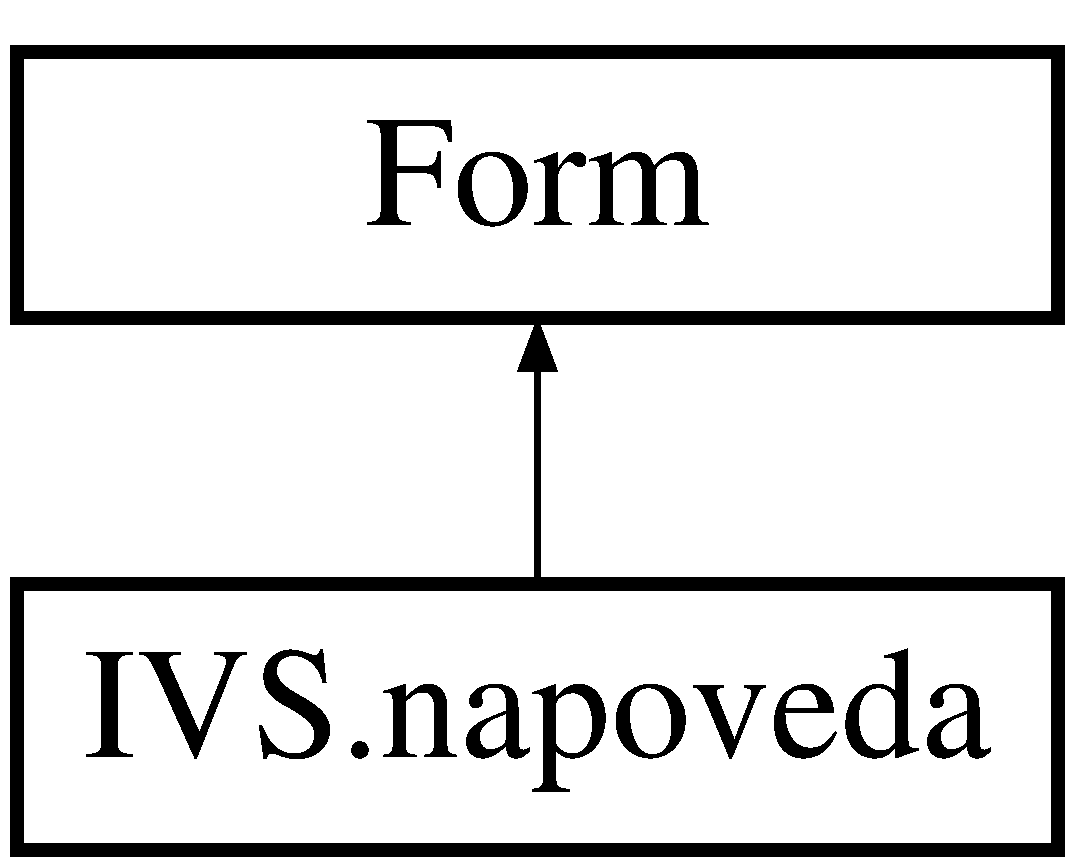
\includegraphics[height=2.000000cm]{class_i_v_s_1_1napoveda}
\end{center}
\end{figure}
\subsection*{Public Member Functions}
\begin{DoxyCompactItemize}
\item 
\mbox{\hyperlink{class_i_v_s_1_1napoveda_a97471343e0e827c2f75fc4c64937f515}{napoveda}} ()
\begin{DoxyCompactList}\small\item\em Init komponent \end{DoxyCompactList}\end{DoxyCompactItemize}
\subsection*{Protected Member Functions}
\begin{DoxyCompactItemize}
\item 
override void \mbox{\hyperlink{class_i_v_s_1_1napoveda_aeec632e7bb98b05061ff7ab39373ef4b}{Dispose}} (bool disposing)
\begin{DoxyCompactList}\small\item\em Clean up any resources being used. \end{DoxyCompactList}\end{DoxyCompactItemize}


\subsection{Detailed Description}
Trida formulare napovedy 



\subsection{Constructor \& Destructor Documentation}
\mbox{\Hypertarget{class_i_v_s_1_1napoveda_a97471343e0e827c2f75fc4c64937f515}\label{class_i_v_s_1_1napoveda_a97471343e0e827c2f75fc4c64937f515}} 
\index{I\+V\+S\+::napoveda@{I\+V\+S\+::napoveda}!napoveda@{napoveda}}
\index{napoveda@{napoveda}!I\+V\+S\+::napoveda@{I\+V\+S\+::napoveda}}
\subsubsection{\texorpdfstring{napoveda()}{napoveda()}}
{\footnotesize\ttfamily I\+V\+S.\+napoveda.\+napoveda (\begin{DoxyParamCaption}{ }\end{DoxyParamCaption})}



Init komponent 



\subsection{Member Function Documentation}
\mbox{\Hypertarget{class_i_v_s_1_1napoveda_aeec632e7bb98b05061ff7ab39373ef4b}\label{class_i_v_s_1_1napoveda_aeec632e7bb98b05061ff7ab39373ef4b}} 
\index{I\+V\+S\+::napoveda@{I\+V\+S\+::napoveda}!Dispose@{Dispose}}
\index{Dispose@{Dispose}!I\+V\+S\+::napoveda@{I\+V\+S\+::napoveda}}
\subsubsection{\texorpdfstring{Dispose()}{Dispose()}}
{\footnotesize\ttfamily override void I\+V\+S.\+napoveda.\+Dispose (\begin{DoxyParamCaption}\item[{bool}]{disposing }\end{DoxyParamCaption})\hspace{0.3cm}{\ttfamily [protected]}}



Clean up any resources being used. 


\begin{DoxyParams}{Parameters}
{\em disposing} & true if managed resources should be disposed; otherwise, false.\\
\hline
\end{DoxyParams}


The documentation for this class was generated from the following files\+:\begin{DoxyCompactItemize}
\item 
I\+V\+S/napoveda.\+cs\item 
I\+V\+S/napoveda.\+Designer.\+cs\end{DoxyCompactItemize}

\hypertarget{class_smerodatna__odhylka_1_1_program}{}\section{Smerodatna\+\_\+odhylka.\+Program Class Reference}
\label{class_smerodatna__odhylka_1_1_program}\index{Smerodatna\+\_\+odhylka.\+Program@{Smerodatna\+\_\+odhylka.\+Program}}


The documentation for this class was generated from the following file\+:\begin{DoxyCompactItemize}
\item 
Smerodatna odhylka/Program.\+cs\end{DoxyCompactItemize}

\hypertarget{class_i_v_s_1_1_testy}{}\section{I\+V\+S.\+Testy Class Reference}
\label{class_i_v_s_1_1_testy}\index{I\+V\+S.\+Testy@{I\+V\+S.\+Testy}}
Inheritance diagram for I\+V\+S.\+Testy\+:\begin{figure}[H]
\begin{center}
\leavevmode
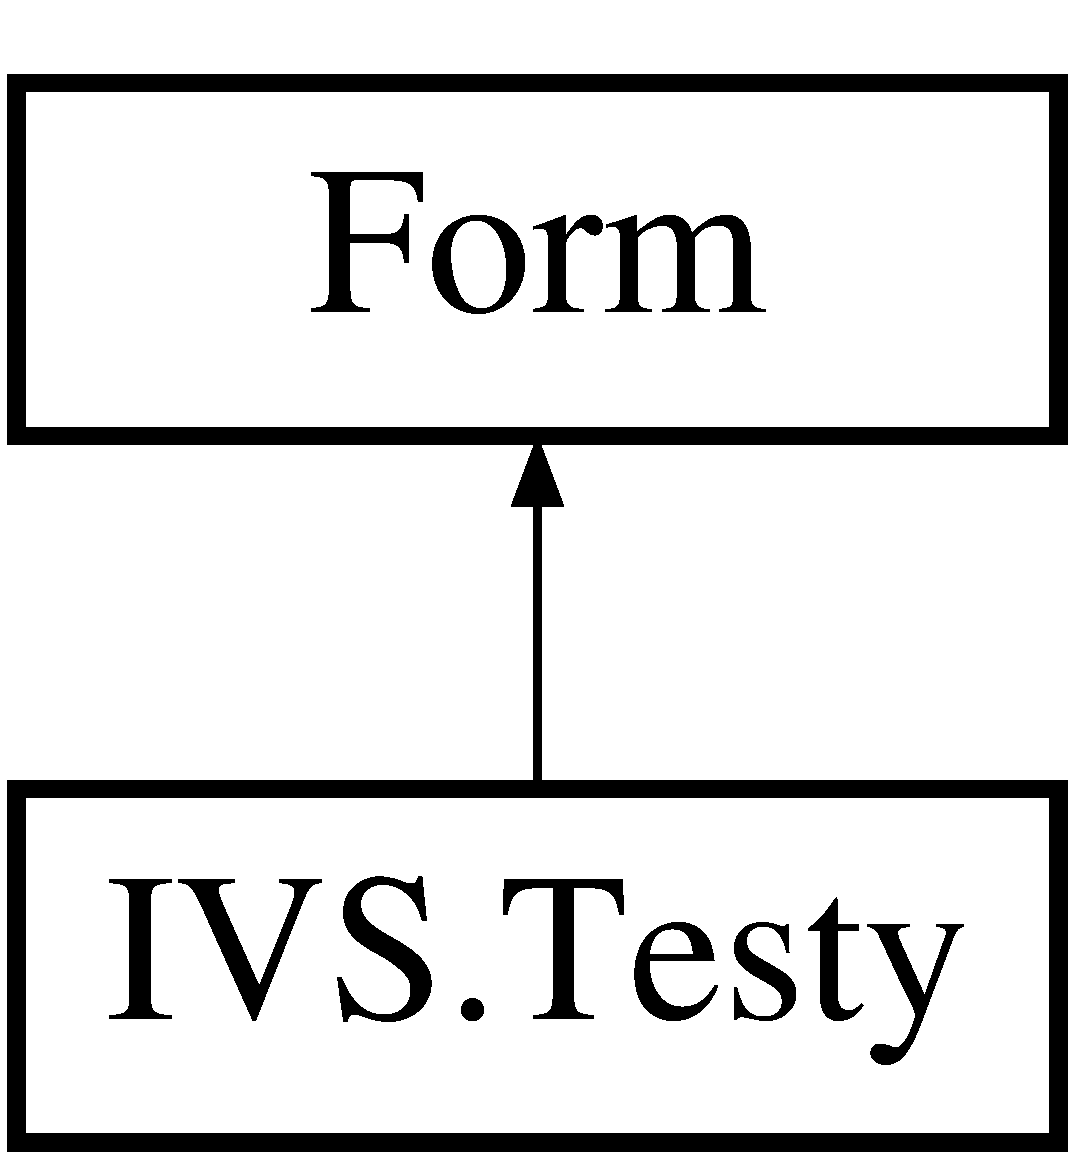
\includegraphics[height=2.000000cm]{class_i_v_s_1_1_testy}
\end{center}
\end{figure}
\subsection*{Public Member Functions}
\begin{DoxyCompactItemize}
\item 
\mbox{\hyperlink{class_i_v_s_1_1_testy_aa23cf506d76f5bc99002eeae9fd2f91c}{Testy}} ()
\begin{DoxyCompactList}\small\item\em Vytvoreni noveho objektu, provedeni testu \end{DoxyCompactList}\end{DoxyCompactItemize}
\subsection*{Protected Member Functions}
\begin{DoxyCompactItemize}
\item 
override void \mbox{\hyperlink{class_i_v_s_1_1_testy_a231cc8b0d786365ab6a36d8e7ef902aa}{Dispose}} (bool disposing)
\begin{DoxyCompactList}\small\item\em Clean up any resources being used. \end{DoxyCompactList}\end{DoxyCompactItemize}


\subsection{Constructor \& Destructor Documentation}
\mbox{\Hypertarget{class_i_v_s_1_1_testy_aa23cf506d76f5bc99002eeae9fd2f91c}\label{class_i_v_s_1_1_testy_aa23cf506d76f5bc99002eeae9fd2f91c}} 
\index{I\+V\+S\+::\+Testy@{I\+V\+S\+::\+Testy}!Testy@{Testy}}
\index{Testy@{Testy}!I\+V\+S\+::\+Testy@{I\+V\+S\+::\+Testy}}
\subsubsection{\texorpdfstring{Testy()}{Testy()}}
{\footnotesize\ttfamily I\+V\+S.\+Testy.\+Testy (\begin{DoxyParamCaption}{ }\end{DoxyParamCaption})}



Vytvoreni noveho objektu, provedeni testu 



\subsection{Member Function Documentation}
\mbox{\Hypertarget{class_i_v_s_1_1_testy_a231cc8b0d786365ab6a36d8e7ef902aa}\label{class_i_v_s_1_1_testy_a231cc8b0d786365ab6a36d8e7ef902aa}} 
\index{I\+V\+S\+::\+Testy@{I\+V\+S\+::\+Testy}!Dispose@{Dispose}}
\index{Dispose@{Dispose}!I\+V\+S\+::\+Testy@{I\+V\+S\+::\+Testy}}
\subsubsection{\texorpdfstring{Dispose()}{Dispose()}}
{\footnotesize\ttfamily override void I\+V\+S.\+Testy.\+Dispose (\begin{DoxyParamCaption}\item[{bool}]{disposing }\end{DoxyParamCaption})\hspace{0.3cm}{\ttfamily [protected]}}



Clean up any resources being used. 


\begin{DoxyParams}{Parameters}
{\em disposing} & true if managed resources should be disposed; otherwise, false.\\
\hline
\end{DoxyParams}


The documentation for this class was generated from the following files\+:\begin{DoxyCompactItemize}
\item 
I\+V\+S/Testy.\+cs\item 
I\+V\+S/Testy.\+Designer.\+cs\end{DoxyCompactItemize}

%--- End generated contents ---

% Index
\backmatter
\newpage
\phantomsection
\clearemptydoublepage
\addcontentsline{toc}{chapter}{Index}
\printindex

\end{document}
